\chapter{Minorové operace}

V této kapitole zavedeme operace s klastrovým grafem, které zachovávají klastrovou rovinnost. V závěru kapitoly zavedeme pojem klastrového minoru, jakožto hlavní pojem této kapitoly, jenž v následující kapitole použijeme pro charakterizaci zakázaných minorů omezených problémů klastrové rovinnosti.

\begin{defn} (minorové operace) Mějme klastrový graf $(G, \mathcal C)$. Minorové operace na klastrových grafech jsou následující:

(Pozn.: Pokud se neřekne jinak, operace se smí provést v nakreslené~i~nenakreslené verzi)

\textit{Odebráním vrcholu $v$} z klastrového grafu $(G, \mathcal C)$ vznikne klastrový graf  $(G', \mathcal C')$, kde  $G' = (V \setminus \{v\}, E \setminus \{f |$ hrana $f$ obsahovala vrchol $v\})$ a $\mathcal C'$ je klastrová hierarchie, kde se z klastrů odebere vrchol $v$, pokud v nich byl.

\textit{Odebráním hrany $e$} z klastrového grafu $(G, \mathcal C)$ vznikne klastrový graf  $(G', \mathcal C)$, kde $G' =  (V,E \setminus \{e\})$.

\textit{Odebráním klastru $K$} z klastrového grafu $(G, \mathcal C)$ vznikne klastrový graf  $(G, \mathcal C')$, kde $\mathcal C' = \mathcal C \setminus K$.

\textit{Kontrakcí hrany $e=\{x,y\}$} z klastrového grafu $(G, \mathcal C)$ vznikne klastrový graf  $(G', \mathcal C')$, kde $G'$ je graf, který obdržíme kontrakcí hrany $e$ a $\mathcal C'$ získáme nahrazením vrcholů $x$ a $y$ ve všech klastrech, kde byly, vrcholem vzniklým kontrakcí. Kontrakci můžeme provést za předpokladu, že koncové vrcholy $x, y$ leží ve stejných klastrech.

\textit{Nahrazením klastru $K=\{x,y\}$ o velikosti 2 hranou $e$} z klastrového grafu klastrového grafu $(G, \mathcal C)$ vznikne klastrový graf  $(G', \mathcal C')$, kde $G'=(V,E \cup e)$ a $\mathcal C'= C \setminus K$. Předpokládáme, že vrcholy $x, y$ nejsou spojeny hranou, neboť v tom případě tato operace není potřebná. U nakreslené verze navíc předpokládáme, že $e$ má jednoznačně dané kombinatorické nakreslení.

\textit{Odebráním vrcholu $v$ z klastru $K$} z klastrového grafu $(G, \mathcal C)$ vznikne klastrový graf  $(G, \mathcal C')$, kde $\mathcal C'$ vznikne nahrazením klastru $K$ klastrem $K \setminus \{v\}$. Tuto operaci lze provést za předpokladu, že z vrcholu $v$ vychází právě jedna hrana ven z $K$ a $K$ je nejmenší (vzhledem k inkluzi) klastr obsahující $v$.

\textit{Sjednocení disjuktních klastrů $K_1$ a $K_2$} z klastrového grafu $(G, \mathcal C)$ vznikne klastrový graf  $(G, \mathcal C')$, kde $C'  := (C\setminus \{K_1,K_2\}) \cup \{K_1 \cup K_2\}$. Sjednocení klastrů můžeme provést za předpokladů, že $K_1, K_2$ jsou dva minimální klastry (nemají podklastry) se společným rodičem, $K_1 \cup K_2$ neindukuje kružnici s vrcholem mimo $K_1 \cup K_2$ uvnitř. Jinými slovy $K_1 \cup K_2$ nemá díru v $G$ (v nakreslené verzi). V nenakreslené verzi je podmínkou, že existuje nakreslení $\rho$ grafu $G$ takové, že $K_1 \cup K_2$ nemá díru v $\rho$. Posledním předpokladem je, že existuje hrana spojující $K_1$ s $K_2$.
\end{defn}

Název minorové operace je užit proto, že každá operace zjednodušuje daný vstupní klastrový graf. U sjednocení klastrů v nenakresleném klastrovém grafu je obtížné říci, kdy potřebné nakreslení existuje, to činí operaci méně použitelnou.
Nyní vyzkoumáme dopad minorových operací na klastrový graf, konkrétně dopad na existenci klastrového nakreslení. Kromě nahrazení klastru hranou můžeme uvážit i nahrazení hrany klastrem velikosti 2. To můžeme provést v případě, že konce hrany patří do stejných klastrů.

\begin{tvr} Nechť $(G', \mathcal C')$ vznikne z $(G, \mathcal C)$ minorovou operací. Potom pokud $(G, \mathcal C)$ je klastrově rovinný, tak $(G', \mathcal C')$ je klastrově rovinný.
\label{min_op_zach_kl_rov}
\end{tvr}
\begin{proof}

Mějme klastrový graf $(G, \mathcal C)$ a jeho klastrové nakreslení $\rho$.

Odebrání vrcholu, hrany či klastru zachovává klastrovou rovinnost:\\
Mějme dáno klastrové nakreslení. Odebrání hrany zapříčiní jedině to, že se nemusí v daném nakreslení hrana kreslit. Podobně pro odebraný vrchol, kdy se odeberou hrany vedoucí do něj. Odebraný klastr se též prostě nenakreslí.

Kontrakce hrany zachovává klastrovou rovinnost:\\
Mějme dáno klastrové nakreslení. Kontrakce je jen vlastně smrštění hrany do jediného bodu, jenž zastupuje vrchol vzniklý kontrakcí.

Nahrazení klastru $K=\{x,y\}$ hranou $e$ zachovává klastrovou rovinnost:\\
Jelikož $(G, \mathcal C)$ je klastrově rovinný, tak máme saturátor $S$. Jelikož $K$ je podle předpokladu nesouvislý, tak po přidání saturátoru jsou vrcholy $x, y$ spojeny hranou. Tato hrana ze saturátoru spojující $x,y$ je hledanou hranou $e$. V nakreslené verzi je požadavek na jednoznačnost, protože by se jinak mohlo stát, že nahrazením klastru hranou vznikne díra.  

Odebrání vrcholu z klastru zachovává klastrovou rovinnost:\\
Jednoduchý překreslovací argument, kdy podél hrany protáhneme hranici klastru až ji přetáhneme přes vyjímaný vrchol.

Sjednocení klastrů zachovává klastrovou rovinnost:\\
Nechť $S$ je minimální saturátor $(G,\mathcal C)$ takový, že $(G \cup S,\mathcal C)$ nemá díru. $S$ je saturátorem i pro klastrový graf $(G, \mathcal C')$, kde ale může být díra.
Nechť $S'$ je minimální saturátor $(G, \mathcal C')$ a $S' \subseteq S$. Tvrdíme, že $(G \cup S',\mathcal C')$ nemá díru. To dokážeme sporem.

Nechť $D$ je díra. Ta musí být ve sjednocení klastrů $K_1$ a $K_2$, neboť kdyby byla jinde, bylo by to ve sporu s předpokladem, že $(G \cup S, \mathcal C)$ nemá díru.
Díra $D$ má neprázdný průnik se saturátorem $S'$. Kdyby průnik byl prázdný, znamenalo by to, že příslušná díra byla v původním klastrovém grafu. Označme tuto hranu $e = \{x,y\}$, kde $x$ a $y$ jsou její koncové vrcholy.
Jako $S''$ označme $S' \setminus e$. Množina $S''$ je saturátorem, protože každý klastr $K \in C$ obsahující vrcholy  $x$ a $y$ obsahuje i cestu $D \setminus \{e\}$. Dostali jsme tedy spor s minimalitou $S'$. $S'$ tedy neobsahuje díry.
\end{proof}

Sjednocení klastrů má dost přepokladů, a proto uvedeme, proč jsou tyto předpoklady nutné. Předpoklad o společném rodiči je z důvodu zachování klastrové hierarchie. Klastrový graf z obrázku \ref{podklastr} ukazuje, proč je nutný předpoklad o tom, že sjednocované klastry nesmějí mít podklastry.

\begin{figure}[H]
\centering
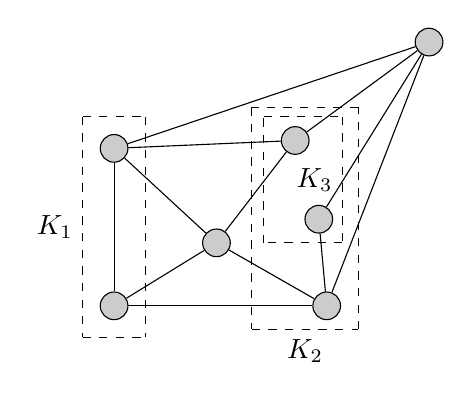
\begin{tikzpicture}[node/.style={circle,fill=black!20,draw,minimum size=1em,inner sep=3pt]}]
  
  \node[node] (1) at  (0,0) {};
  \node[node] (2) at  (0,-2) {};
  \node[node] (3) at  (1.3,-1.2) {};
  \node[node] (4) at  (2.3,0.1) {};
  \node[node] (5) at  (2.6,-0.9) {};
  \node[node] (6) at  (2.7,-2) {};
  \node[node] (7) at  (4,1.35) {};

  \draw (1) -- (2);
  \draw (1) -- (3);
  \draw (1) -- (4);
  \draw (1) -- (7);
  \draw (2) -- (3);
  \draw (2) -- (6);
  \draw (3) -- (4);
  \draw (3) -- (6);
  \draw (4) -- (7);
  \draw (5) -- (6);
  \draw (5) -- (7);
  \draw (6) -- (7);

  \draw[dashed] (-0.4,0.4) to node [auto,swap] {$K_1$} (-0.4,-2.4);
  \draw[dashed] (-0.4,0.4) -- (0.4,0.4);
  \draw[dashed] (0.4,0.4) -- (0.4,-2.4);
  \draw[dashed] (-0.4,-2.4) -- (0.4,-2.4);

  \draw[dashed] (1.9,-1.2) -- (1.9,0.4);
  \draw[dashed] (1.9,0.4) -- (2.9,0.4);
  \draw[dashed] (2.9,0.4)  to node [auto,swap] {$K_3$} (2.9,-1.2);
  \draw[dashed] (2.9,-1.2) -- (1.9,-1.2);

  \draw[dashed] (1.75,-2.3) to node [auto,swap] {$K_2$} (3.1,-2.3);
  \draw[dashed] (3.1,-2.3) -- (3.1,0.52);
  \draw[dashed] (3.1,0.52) --  (1.75,0.52);
  \draw[dashed]  (1.75,0.52) -- (1.75,-2.3);
\end{tikzpicture}
\caption{Klastr $K_3$ brání sjednocení klastrů $K_1$ a $K_2$, neboť jeho saturováním (nahrazení hranou) by v $K_1 \cup K_2$ vznikla díra. Kdybychom vynechali $K_3$, pak už je snadné najít klastrové nakreslení.}
\label{podklastr}
\end{figure}

Nyní se podíváme na dva speciální případy sjednocení klastrů. Jeden případ je přidání vrcholu do klastru, který je vlastně inverzí k odebrání vrcholu z klastru. 

\begin{tvr} Mějme klastrový graf $(G, \mathcal C)$ a vrchol $v \in V(G)$ a klastr $K \in \mathcal C$. Nechť $K$ neobsahuje podklastry a každý klastr obsahující $v$ obsahuje i $K$, $v$ sousedí s $K$, tedy $v$ je spojen s nějakým vrcholem v $K$ hranou a
$K \cup \{v\}$ neindukuje kružnici s vrcholem mimo $K$ uvnitř.
$\mathcal C' = (\mathcal C \setminus \{K\}) \cup \{ K \cup \{v\} \}$
Potom $(G, \mathcal C)$ je klastrově rovinný $\implies (G, \mathcal C')$ je klastrově rovinný.
\end{tvr}
\begin{proof}
Jednoduše budeme vrchol vydávat za jednovrcholový klastr. Zbytek plyne z toho, že sjednocení zachovává klastrovou rovinnost, jelikož jsou splněny všechny předpoklady.
\end{proof}

Podobně pro nenakreslenou verzi. Druhý případ je, když klastry spojuje právě jedna hrana. Tento případ nám dává příklad, kdy můžeme provést sjednocení klastrů i pro nenakreslené klastrové grafy.
\begin{tvr}
Mějme klastrový graf  $(G, \mathcal C)$ a dva disjunktní klastry $K_1$ a $K_2$, které spojuje právě jedna hrana $e$. Nechť $K_1$ a $K_2$ mají společného rodiče a nemají podklastry. Mějme klastrový graf $(G, \mathcal C')$, kde  $\mathcal C'  := (\mathcal C \setminus \{K_1,K_2\}) \cup \{K_1 \cup K_2\}$. Potom $(G, \mathcal C)$ je klastrově rovinný $\implies (G, \mathcal C')$ je klastrově rovinný.
\end{tvr}
\begin{proof}
Pro použití výsledku o sjednocení klastrů nám stačí ukázat, že $K_1 \cup K_2$ neobsahuje díru. Protože klastry $K_1$ a $K_2$ spojuje právě jedna hrana, tak jediné kružnice ve sjednocení jsou buď $K_1$ nebo v $K_2$. Podle předpokladu, že $(G, \mathcal C)$ je klastrově rovinný, tak $K_1$ ani $K_2$ neobsahují díru. Podle tvrzení \ref{min_op_zach_kl_rov} je $\implies (G, \mathcal C')$ klastrově rovinný.
\end{proof}

Vyzbrojeni minorovými operacemi můžeme definovat pojem klastrového minoru.

\begin{defn}
Mějme klastrový graf $(G,\mathcal C)$. Klastrový graf $(G',\mathcal C')$ je klastrovým minorem, pokud jej lze získat konečnou posloupností minorových operací z klastrového grafu $(G,\mathcal C)$.
\end{defn}

\begin{dusl} Klastrový minor klastrově rovinného klastrového grafu je klastrově rovinný.
\label{důsledek}
\end{dusl}
\begin{proof}
Důkaz se provede indukcí podle délky posloupnosti, kde se využije toho, že minorové operace zachovávají klastrovou rovinnost.
\end{proof}